\chapter{Methodology}
\section{System Design}
The project focuses on the implementation of an algorithm that can detect disturbance in crowd. It considers how flow-vector magnitudes change over time, which are collected for short frame sequences, and then classified as either normal or abnormal situation using a classifier.
\par
The aim of the project is to keep the processing very quick, a detection should be made within a few seconds of the outbreak of violence. It has to detect the change of normal behaviour to abnormal behaviour with the shortest delay from the time that the change has occurred.

\begin{figure}[H]
\centering
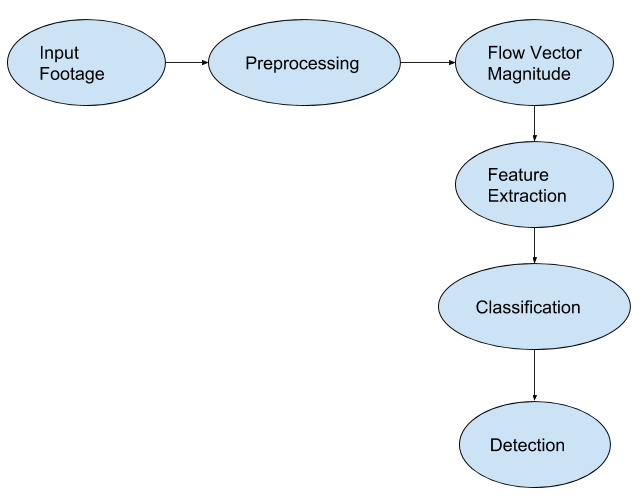
\includegraphics[scale = 0.4]{system_design.png}
\caption{System Design}
\end{figure}

\section{Implementation of Proposed Solution}
\subsection{Input Footage}
For training of the classifier input of the footage will be from a fixed dataset. For practical real time implementation footage from externally attached cameras can be used. The resolution of the input footage need not be specific. Generally the resolution of a CCTV footage is of 704 X 480 pixels. This proposed algorithm reduces the height of the video to 100 pixels and width accordingly. This increases the scalability of the algorithm. Even high definition videos can be processed with the proposed algorithm.
\subsection{Preprocessing}
Preprocessing the input data is very important part of the algorithm. Optical flow algorithm will take at least one minute to calculate optical flow of a high definition image. So as to constraint the processing to real time preprocessing must done. As mentioned earlier any image is being resized to 100 pixel height and respective width accordingly. Preprocessing is done in a way such that the aspect ratio of the video is not disturbed.
\subsection{Flow Vector Magnitude}
For each pixel in the video has some velocity corresponding to it, along x direction and y direction. The Flow Vector Magnitude is nothing but the magnitudes of these velocities. Computing Flow Vector Magnitude is computationally heavy, this is the most time taking part of the proposed algorithm. Since we are reducing the size of frames considerably, this is computation is quick enough to cope us with real time violence detection.
\subsection{Feature Extraction}
Feature extraction is based on the computation of ViF (Violence Flow Descriptors). These descriptors are quantised values of the above generated Flow Vector Magnitudes. After ViF is generated a histogram is built which will assign different ViF values to corresponding bins in the range of (0 to 1.0) with the intervals of 0.05, i.e 20 bins.
\subsection{Classification}
After the features have been extracted, classification can done with the help of a simple Linear SVM. So as to further increase the accuracy of the algorithm , SVM with AdaBoost can be used. For our project a trained neural net has been used since it is providing a better accuracy.
\subsection{Detection}
Detection in a video footage is the final output of the proposed algorithm. It is taking place with the help classifier model that is being trained in the above step. According to the base paper, a sequence of 10 frames i.e on an average two-fifth of a second is enough to detect violence in a footage. Detection may be further improved continuous learning in real-time also.
\section{Languages and Tools}
Only open source languages and tools are used in developing the project. Unix environment is being used for the development of the process.
\subsection{Language}
Language used is Python and the main tool used is OpenCV for video processing. Python is interpreted language which is used for general-purpose programming. It is a user-friendly language which emphasizes on code readability and its syntax allows users to write programs with relatively fewer lines of code when compared to C/C++, Java etc. Python 2.7 version is used in the project.\\
Python's \textbf{features} include:
\begin{itemize}
\item Easy-to-learn: Python has few keywords, simple structure, and a clearly defined syntax. This allows the student to pick up the language quickly.
\item Easy-to-read: Python code is more clearly defined and visible to the eyes.
\item Easy-to-maintain: Python's source code is fairly easy-to-maintain.
\item A broad standard library: Python's bulk of the library is very portable and cross-platform compatible on UNIX, Windows, and Macintosh.
\item Interactive Mode: Python has support for an interactive mode which allows interactive testing and debugging of snippets of code.
\item Portable: Python can run on a wide variety of hardware platforms and has the same interface on all platforms.
\item Extendable: You can add low-level modules to the Python interpreter. These modules enable programmers to add to or customize their tools to be more efficient.
\item Databases: Python provides interfaces to all major commercial databases.
\item GUI Programming: Python supports GUI applications that can be created and ported to many system calls, libraries and windows systems, such as Windows MFC, Macintosh, and the X Window system of Unix.
\item Scalable: Python provides a better structure and support for large programs than shell scripting.
\end{itemize}
Apart from the above-mentioned features, Python has a big list of good features, few are listed below:
\begin{itemize}
	\item It supports functional and structured programming methods as well as OOP.
\item It can be used as a scripting language or can be compiled to byte-code for building large applications.
\item It provides very high-level dynamic data types and supports dynamic type checking.
\item It supports automatic garbage collection.
\item It can be easily integrated with C, C++, COM, ActiveX, CORBA, and Java.

\end{itemize}
\subsection{OpenCV}
OpenCV (Open Source Computer Vision Library) is an open source computer vision and machine learning software library. OpenCV was built to provide a common infrastructure for computer vision applications and to accelerate the use of machine perception in the commercial products. Being a BSD-licensed product, OpenCV makes it easy for businesses to utilize and modify the code.\par
The library has more than 2500 optimized algorithms, which includes a comprehensive set of both classic and state-of-the-art computer vision and machine learning algorithms. These algorithms can be used to detect and recognize faces, identify objects, classify human actions in videos, track camera movements, track moving objects, extract 3D models of objects, produce 3D point clouds from stereo cameras, stitch images together to produce a high resolution image of an entire scene, find similar images from an image database, remove red eyes from images taken using flash, follow eye movements, recognize scenery and establish markers to overlay it with augmented reality, etc. OpenCV has more than 47 thousand people of user community and estimated number of downloads exceeding 14 million. The library is used extensively in companies, research groups and by governmental bodies.\par
Along with well-established companies like Google, Yahoo, Microsoft, Intel, IBM, Sony, Honda, Toyota that employ the library, there are many start-ups such as Applied Minds, VideoSurf, and Zeitera, that make extensive use of OpenCV. OpenCV’s deployed uses span the range from stitching street view images together, detecting intrusions in surveillance video in Israel, monitoring mine equipment in China, helping robots navigate and pick up objects at Willow Garage, detection of swimming pool drowning accidents in Europe, running interactive art in Spain and New York, checking runways for debris in Turkey, inspecting labels on products in factories around the world on to rapid face detection in Japan.\par
OpenCV is written in C++ and its primary interface is in C++, but it still retains a less comprehensive though extensive older C interface. There are bindings in Python, Java and MATLAB/OCTAVE. The API for these interfaces	can be found in the online documentation. Wrappers in other languages such as C-sharp, Perl, Ch, Haskell and Ruby have been developed to encourage adoption by a wider audience. All the new developments and algorithms in OpenCV are now developed in the C++ interface.\\
There are many \textbf{applications} of OpenCV. A few of them are cited as below:
\begin{itemize}
\item 2D and 3D feature toolkits 
\item Facial recognition system 
\item Gesture recognition 
\item Human–computer interaction (HCI) 
\item Mobile robotics 
\item Motion understanding 
\item Object identification 
\item Segmentation and recognition 
\item Stereopsis stereo vision: depth perception from 2 cameras 
\item Structure from motion (SFM) 
\item Motion tracking 
\end{itemize}

\subsection{Other libraries}
Along with OpenCV we have used bob. Bob is a machine learning platform used in python, it helped us to port Matlab code of optical flow to python. Scikit learn is Python package which is similar to WEKA tool for java. It will be used for training a classifier model in the proposed algorithm of the project.


